\begin{figure}[H]
    \centering
    \vspace{-0.5em}
    \begin{minipage}{0.75\textwidth}
        \centering
        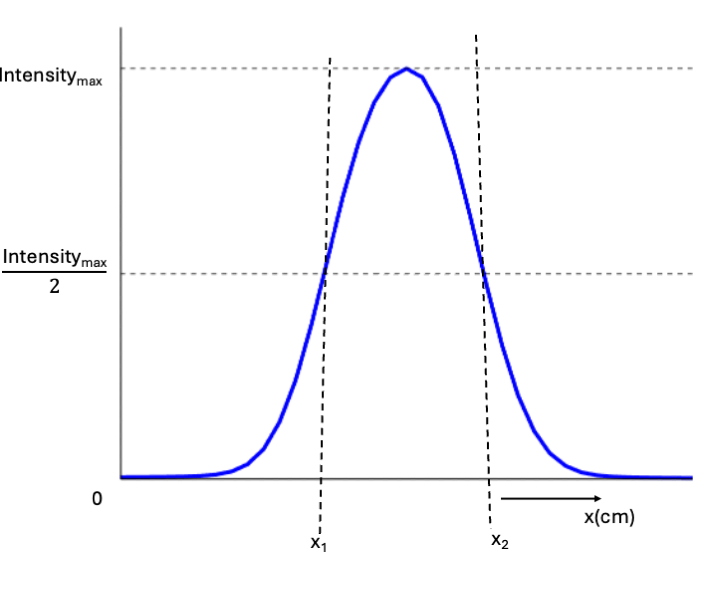
\includegraphics[width=\linewidth]{figures/fwhm_plots.png}
        \vspace{-3em}
        \caption{\textbf{Illustration of the full width at half maximum (FWHM) method used to 
        estimate diffusion distance}. The curve represents fluorescence intensity as a 
        function of position $x$ (cm). The FWHM is defined as the width of the curve at half of 
        its peak intensity, measured between points $x_1$ and $x_2$.}
        \label{fig:full_width_half_maximum}
    \end{minipage}
\end{figure}

